\documentclass[12pt]{article}


\usepackage[dvips,letterpaper,margin=0.75in,bottom=0.5in]{geometry}
\usepackage{cite}
\usepackage{slashed}
\usepackage{graphicx}
\usepackage{amsmath}

\begin{document}

\title{Addendum to Moore's Treatment of Complex Numbers}
\author{Michael Mulhearn}

\maketitle

\section{The Imaginary Unit}

The imaginary unit $i$ is defined by its property:
\begin{equation} \label{eqn:iunit}
i^2 = -1.
\end{equation}
It is somewhat whimsically called the imaginary unit because there is no real number with this property.
This definition of $i$ is in a sense ambiguous, as a quick calculation
\begin{displaymath} 
(-i)^2 = (-1 \cdot i)^2 \cdot (i)^2 = -1.
\end{displaymath}
shows that there are at least two entities with the ``defining''
property their square is $-1$.   This leads to some ambiguity.  For instance, many authors (like Moore) define
\begin{displaymath} 
i = \sqrt{-1}
\end{displaymath} 
but this is a bit perilous, as you can easily be led astray with calculations like:
\begin{displaymath} 
-1 = i^2 = (\sqrt(-1) \cdot \sqrt(-1))^2 = (\sqrt(-1 \cdot -1))^2 = (1)^2 = 1 
\end{displaymath} 
or
\begin{displaymath} 
\frac{1}{i} = \frac{1}{\sqrt{-1}} = \sqrt{\frac{1}{-1}} =  \sqrt{-1} = i.
\end{displaymath}
To avoid ambiguity, one should always treat $i$ as an unknown quantity, with the
property that $i^2=-1$.  So, for instance:
\begin{displaymath} 
\frac{1}{i} = \frac{1}{i} \cdot  \frac{i}{i} = \frac{i}{i^2} = \frac{i}{-1} = -i. 
\end{displaymath}

\section{Complex Numbers}

\begin{figure}[thb]
\begin{center}
{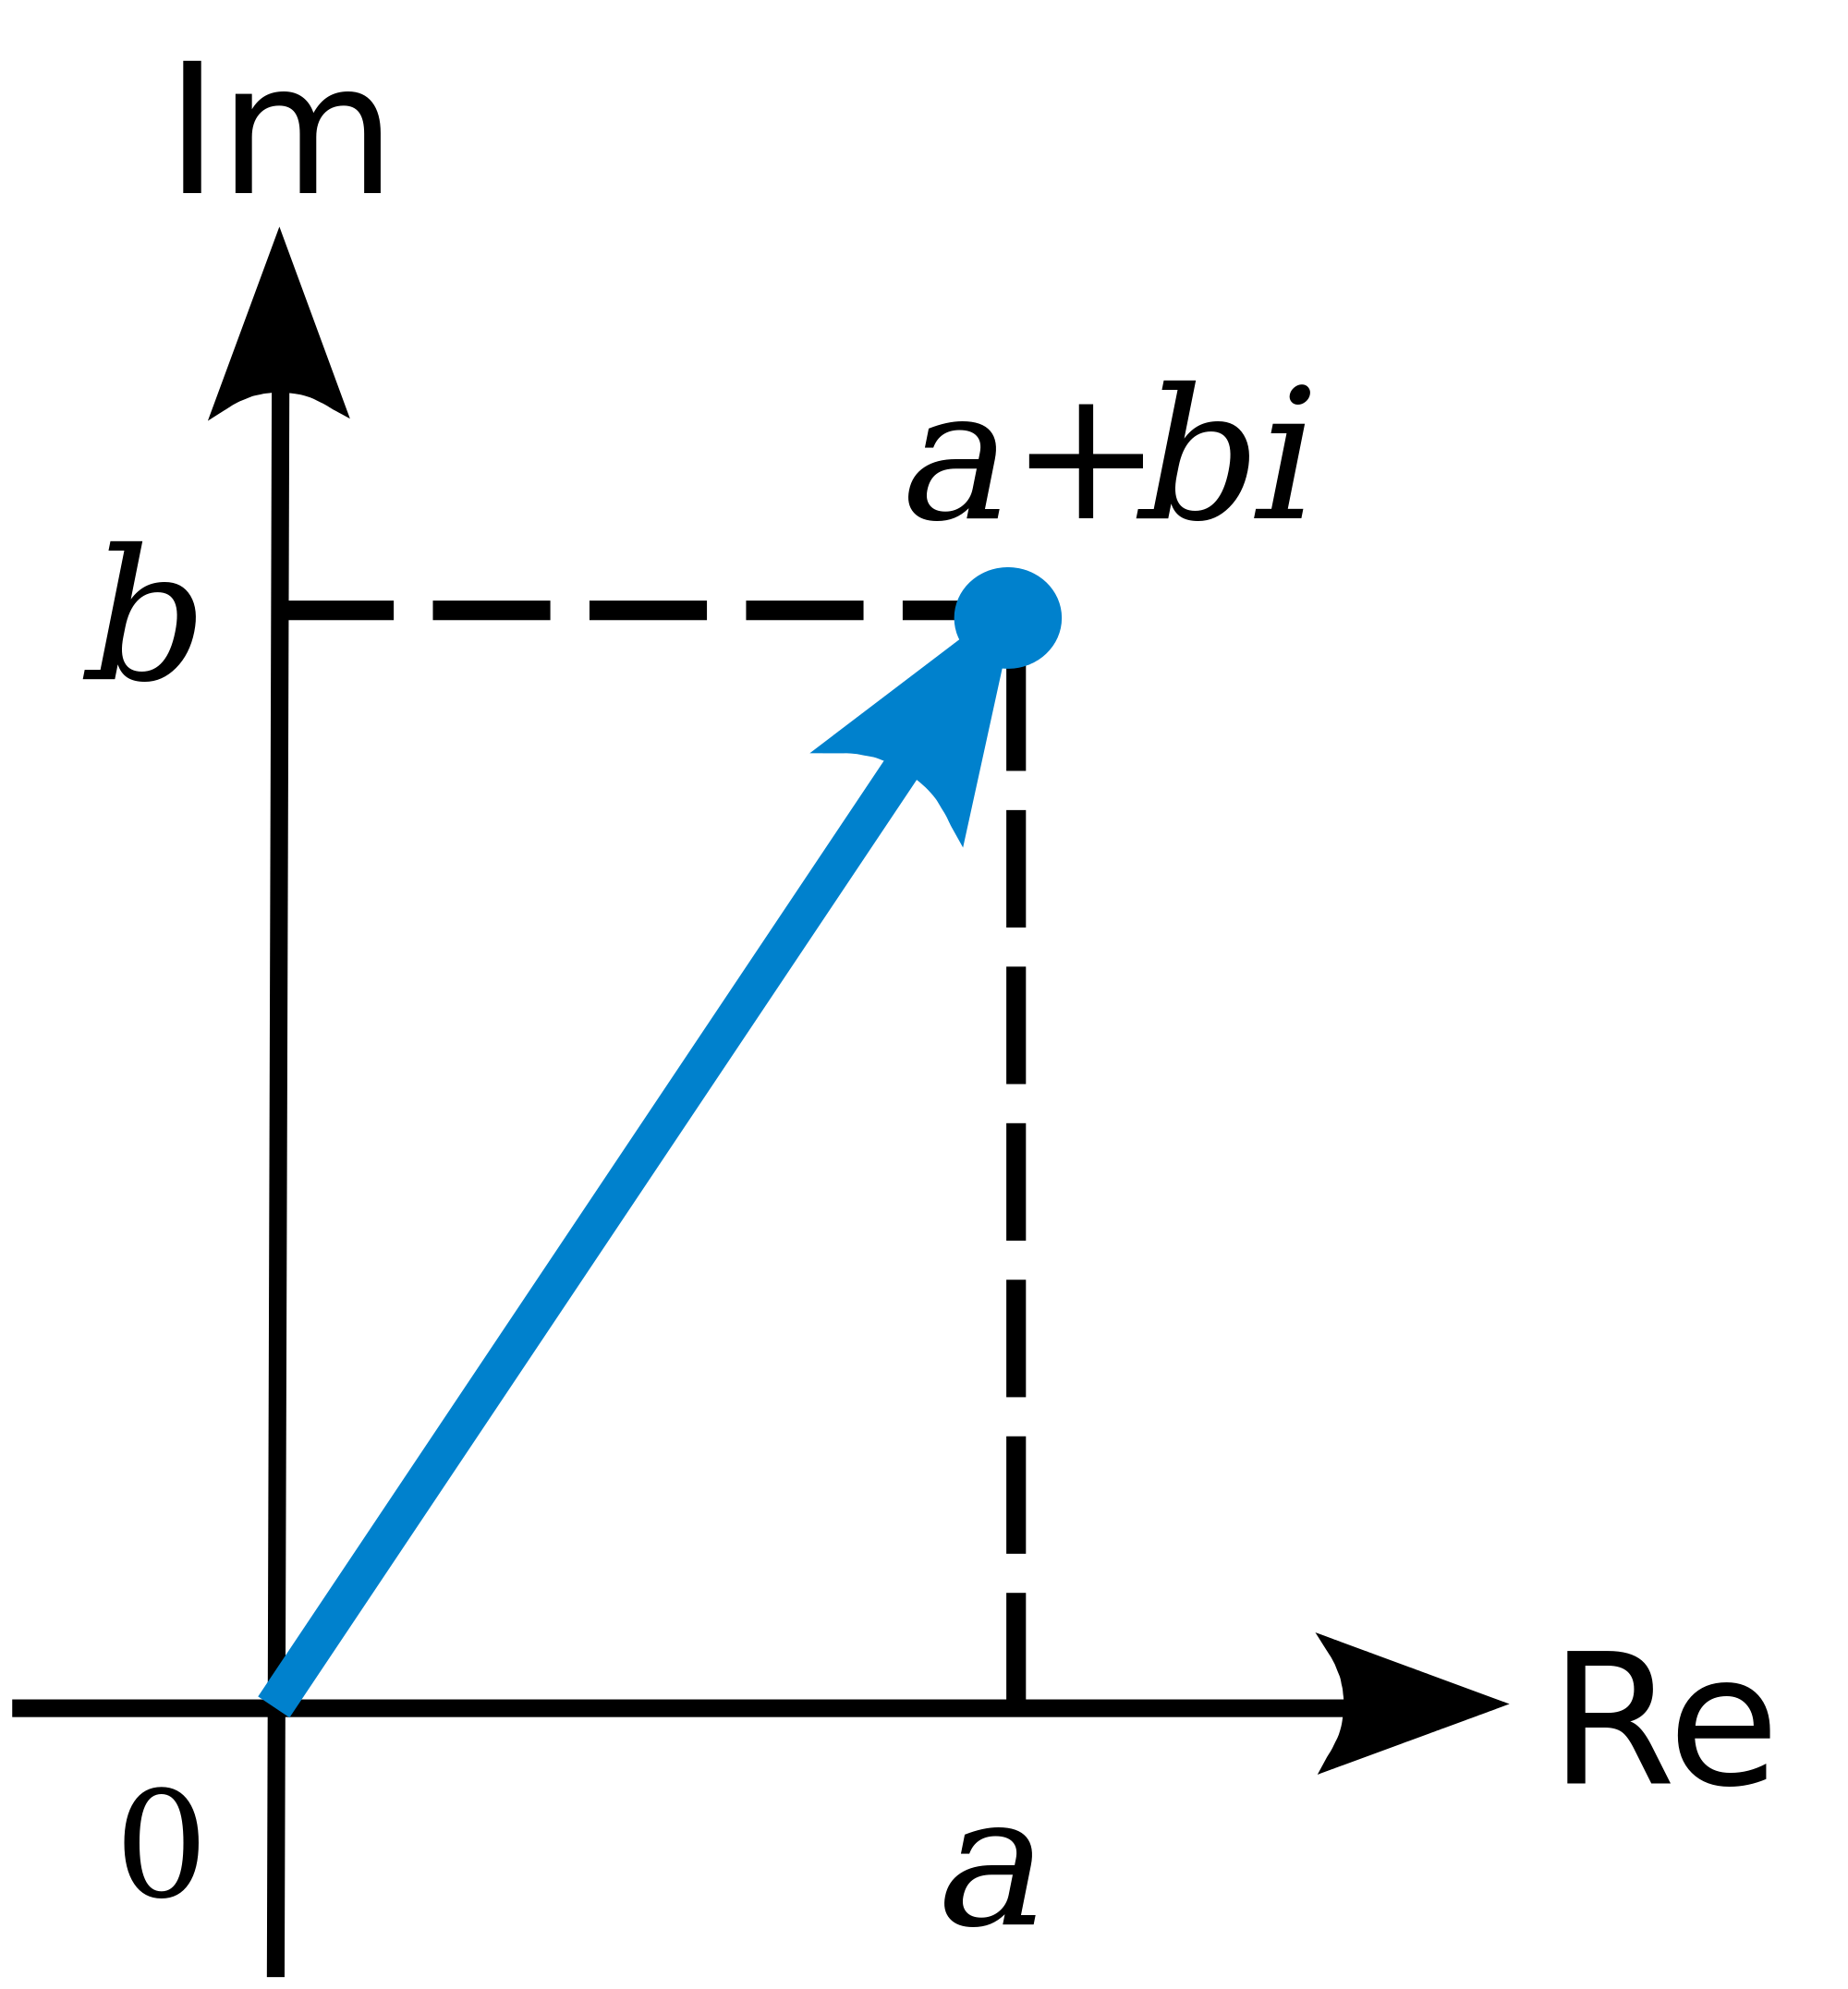
\includegraphics[width=0.30\textwidth]{figs/complex_numbers.png}}
\end{center}
\caption{\label{fig:complexplane} The complex plane}
\end{figure}

A complex number $z$ is constructed from two real numbers $a$ and $b$ as the quantity
\begin{equation} \label{eqn:complex}
z = a + i b 
\end{equation}.
We call $a$ the real part of $z$, and $b$ the imaginary part of $z$, and define the functions:
\begin{eqnarray*}
\Re(a + bi) & = & a \\
\Im(a + bi) & = & b
\end{eqnarray*}

If we have any two complex numbers
\begin{eqnarray*}
z_1 & = &  a_1 + i b_1 \\
z_2 & = &  a_2 + i b_2 \\
\end{eqnarray*}
we define addition, subtraction and multiplication by:
\begin{eqnarray*}
z_1 + z_2 & = &  (a_1 + a_2)+ i (b_1 + b_2) \\
z_1 - z_2 & = &  (a_1 - a_2)+ i (b_1 - b_2) \\
z_1 z_2 & = &  (a_1 + i b_1) \cdot (a_2 + i b_2)  = (a_1 a_2 - b_1 b_2) + i(a_2 b_1 + a_1 b_2)
\end{eqnarray*}
With this definition of multiplication, $i^2 = -1$, as is necessary for self-consistency.

With addition and subtraction defined, we can now define complex conjugate of a complex number $z = a+ib$ by the symbol and definition:
\begin{eqnarray*}
z^* = a - i b
\end{eqnarray*}.  
We define the absolute square of a complex number by
\begin{equation*}
|z|^2  =  z \cdot z^* = a^2 + b^2 \\
\end{equation*}
and its absolute value by
\begin{equation*}
|z|  =  \sqrt{a^2 + b^2}.
\end{equation*}  
Not that both $|z|$ and $|z|^2$ are always positive real numbers.

To calculate the reciprocal of a complex number $z = a+ib$, we convert the denominator to a real number:
\begin{equation*}
\frac{1}{z} = \frac{1}{z} \cdot \frac{z^*}{z^*} = \frac{z^*}{|z|^2} = \left( \frac{a}{a^2+b^2} \right) + i \left( \frac{-b}{a^2+b^2}\right)
\end{equation*}



we can now define complex conjugate of a complex number $z = a+ib$ by the symbol and definition:


\section{Euler's Formula}

\begin{figure}[thb]
\begin{center}
{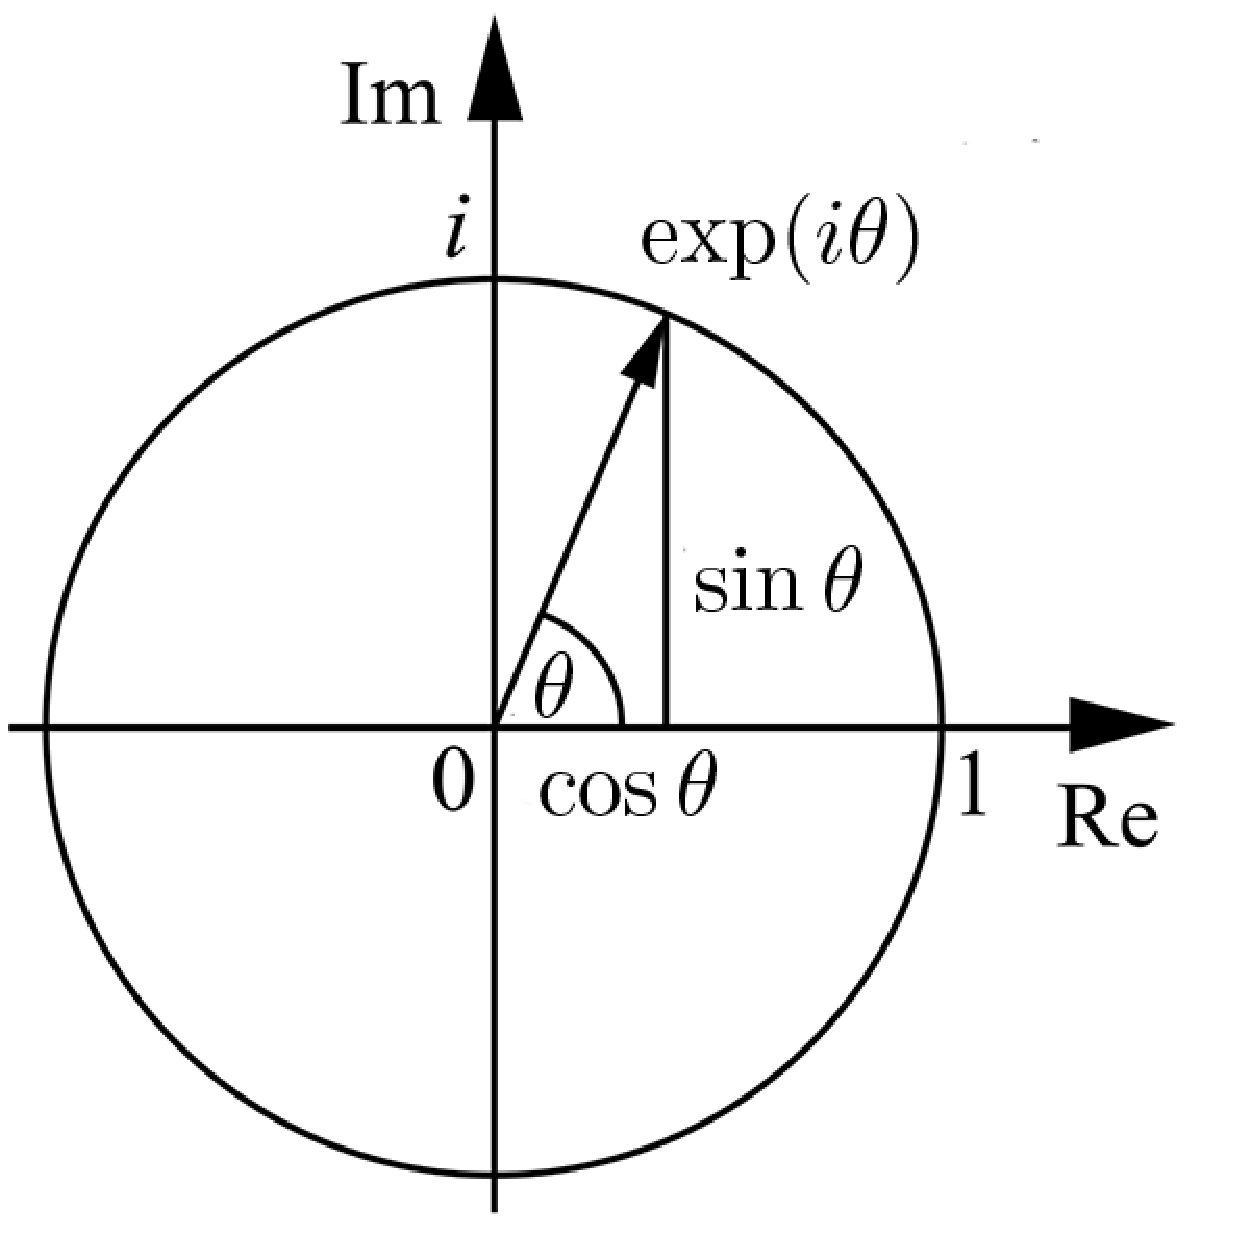
\includegraphics[width=0.30\textwidth]{figs/euler.pdf}}
\end{center}
\caption{\label{fig:euler} The geometric interpretation of the Euler Formula }
\end{figure}

So far we know how to add, subtract, multiply, and divide real numbers.   Next we would like to know how to handle complex exponentials.  Knowing how to handle $\exp(ix)$ will take us quite a distance, because we can certainly write for a real number $A$ raised to a complex number $z=a + ib$
\begin{equation*}
A^z = A^a \cdot A^{ib} = A^a \cdot \exp(ib\ln A)
\end{equation*}
Euler's Formula (not to be confused with Euler's conjectures, numbers, functions, identities,theorems, or laws) is a remarkable prescription for handling $e$ raised to an imaginary power. 

Euler derived his formula by Taylor expanding $\exp(i \theta)$ for some real number $\theta$:
\begin{equation*}
\exp(i\theta) = 1 + i\theta + \frac{i^2 \theta^2}{2} + \frac{i^3 \theta^3}{3!} + \frac{i^4 \theta^4}{4!}
+ \frac{i^5 \theta^5}{5!} + \frac{i^6 \theta^6}{6!} + \frac{i^7 \theta^7}{7!} + ...
\end{equation*}
Now noting that $i^2=-1$, we sort according to the real and imaginary parts:
\begin{equation} \label{eqn:step1}
\exp(i\theta) = \left( 1 - \frac{\theta^2}{2} + \frac{\theta^4}{4!} -  \frac{\theta^6}{6!} + ... \right)
+ i \left( \theta - \frac{\theta^3}{3!} + \frac{\theta^5}{5!} - \frac{\theta^7}{7!} + ... \right)
\end{equation}
The expansions in parenthesis are simple the sine and cosine expansions:
\begin{eqnarray*}
\cos \theta &=& 1 - \frac{\theta^2}{2} + \frac{\theta^4}{4!} -  \frac{\theta^6}{6!} + ... \\
\sin \theta &=& \theta - \frac{\theta^3}{3!} + \frac{\theta^5}{5!} - \frac{\theta^7}{7!} + ... 
\end{eqnarray*}
Identifying these series in Equation~\ref{eqn:step1} results in Euler's remarkable result:
\begin{equation}
\exp(i\theta) = \cos \theta + i \sin \theta
\end{equation}
It is a beautiful result, and it turns out to be exceptionally useful, with widespread application in math,
physics, and engineering.  Much of its utility results in its simple geometric interpretation, depicted in 
Fig.~\ref{fig:euler}.  You will show in the homework that $|z|=1$ for a complex number that can be written 
$z = \exp(i \theta)$.  This places the complex number somewhere on the unit circle $a^2 + b^2 = 1$ in the
complex plane.  The direction $\theta$ specifies the direction of the complex number in polar coordinates.
Changing the value of $\theta$ does not change the magnitude of the complex number $z = \exp(i \theta)$ only its direction.  It is therefore the ideal quantity to describe quantities which interfere due to differing phases.

We can express any complex number in the form:
\begin{displaymath}
z = |z| \exp(i \theta)
\end{displaymath}
We say that $z$ has magnitude $|z|$ and phase $\exp(i \theta)$.  Changing the value of $\theta$ does not change the magnitude of the complex number $z = |z| \exp(i \theta)$ only its direction.  It is therefore the ideal quantity to describe quantities which interfere due to differing phases.


\section{Homework Problems}

%\noindent
%{\em Problem 1:} From the definition of complex conjugation, show that the following properties of complex %conjugation, as reported in Moore, are true
%\begin{eqnarray*}
%(z^*)^* &=& z \\
%(z_1 + z_2)^* &=& z_1^* + z_2^* \\
%(z_1 z_2)^* &=& z_1^* z_2^*
%\end{eqnarray*}  \\

%\vskip 0.5cm

\noindent
{\em Problem 1:} Show that $|\exp(i \theta)| = 1$. \\

\vskip 0.5cm

\noindent
{\em Problem 2:} Show that $\exp(i \theta)^* = \exp(-i \theta)$. \\

\vskip 0.5cm

\noindent
{\em Problem 3:} Derive a formula for division of complex numbers by combining the rules for multiplication and reciprocation.

\vskip 0.5cm

\noindent 
Problems from Moore:\\
Q5:  B9,10 S4,5\\
Q6:  B1, S4,5,7,9 R2\\

\end{document}




